% Build: pdflatex main && bibtex main && pdflatex main && pdflatex main
% Tables and figures come from `python scripts/figures_all.py`. Missing ones show as a red TODO.
\documentclass[conference]{IEEEtran}
\usepackage[T1]{fontenc}
\usepackage{cite}
\usepackage{amsmath}
\usepackage{graphicx}
\usepackage{booktabs}
\usepackage{xcolor}
\usepackage{url}
\usepackage{tikz}
\usetikzlibrary{positioning,arrows.meta,fit}

\newcommand{\todo}[1]{\textcolor{red}{[TODO: #1]}}
\newcommand{\inputtable}[1]{\IfFileExists{tables/#1.tex}{\input{tables/#1.tex}}{\todo{table \detokenize{#1}: run the experiment}}}
\newcommand{\inputfigure}[3]{%
  \IfFileExists{figures/#1.pdf}{%
    \begin{figure#3}[t]\centering\includegraphics[width=\linewidth]{figures/#1.pdf}\caption{#2}\label{fig:#1}\end{figure#3}%
  }{\todo{figure \detokenize{#1}: run the experiment}}}

\begin{document}

\title{Scare First, Reason Later: A Two-Speed Generative-AI Agent for Closed-Loop Crop-Raiding Animal Deterrence from Farm Video}

\author{\IEEEauthorblockN{Mohit Kumar Patwari \todo{confirm author list and order}}
\IEEEauthorblockA{\todo{affiliation, email}}}

\maketitle

\begin{abstract}
\todo{Write last. It must give the real E1--E6 numbers and must say at abstract level that the
deterrence comparison (E4) uses a simulator whose parameters are assumptions, with a field trial
left as future work.}
\end{abstract}

\begin{IEEEkeywords}
crop raiding, human-wildlife conflict, vision-language models, constrained LLM agents, humane deterrence
\end{IEEEkeywords}

\section{Introduction}
\todo{Crop raiding and why the alarm must come before any slow reasoning; state the ``scare first''
requirement. Cite the 19--29\,s and 21--24\,s latencies from Section~\ref{sec:related}.}

Contributions, each tied to a test that could prove it wrong:
\begin{enumerate}
\item \emph{Architecture.} A two-speed design that keeps GenAI off the alarm path (E1).
\item \emph{Retreat verification.} A check, against hand labels, that the animal actually left,
fusing tracker and vision-language model (VLM) evidence (E3).
\item \emph{Outcome-driven deterrence.} An LLM policy constrained to an enum allow-list and a validator,
compared with fixed, random, rule-chain and Thompson-sampling baselines on identical event
streams (E4, simulated, with sensitivity analysis).
\item \emph{Prompting evidence on farm footage.} Multi-frame vs single-frame prompts, location-hint
ablation, local vs cloud VLM (E2).
\item \emph{Farmer communication.} Local-language LLM alerts vs template SMS (E6), plus a released
labelled clip set and code.
\end{enumerate}

\section{Related Work}\label{sec:related}
\subsection{Intrusion detection systems}
Published systems are mostly a detector, a fixed response and a notification, and their response
times leave little room to scare an animal. Shahrir et al.~\cite{shahrir2025hybrid} combine YOLOv5 and SSD
for elephants, boar and monkeys, playing a tiger roar and notifying farmers over Telegram; they train on about
60 images per class, reach mAP 0.965/0.948/0.831 and take 20.8--24.3\,s per inference. The fog-based
system of Miao et al.~\cite{miao2023fog} combines motion sensors, cameras and LoRa; its evaluation uses 18
simulated movements and measures 19.11--28.61\,s in total from detection to farmer alert. Dorji et
al.~\cite{dorji2025bhutan} run YOLOv8 on a Raspberry Pi~4 for seven species, trained on 30,800 images, with
95.7\% accuracy in a controlled laboratory and field validation still to come. WADAS~\cite{repo_wadas}
is an open-source alternative that can drive a deterrent actuator. In our reading, none of these
treats frame-to-alarm latency as a design target or checks what the animal did next.

\subsection{Deterrents and habituation}
Animals learn to tolerate repeated sounds, and the current answer is rule-based variation. Elemantra~\cite{bandara2023elemantra},
for elephants, detects with YOLOv7 on infrared images (537 images; AP$_{50}$ 0.8952 and 0.6752 for its two
model formats) and seismic sensing (recall 0.82), and modifies bee sounds at random (frame-rate change,
pink noise or silent frames) because elephants quickly learn to tolerate them. A ZHAW field study of
wild boar, with 36 GPS-collared animals, used a device that plays alarm and warning calls in random combinations at
irregular intervals, and concluded that no single preventive measure tested offers absolute
protection~\cite{zhaw2019boar}. Evidence for noise against primates is limited: Conservation
Evidence rests its assessment on two studies, and in the Indonesian one noise was applied together with
tree nets (orangutan feeding on crops 69\,min vs 81\,min), so noise cannot be isolated~\cite{ce2026primates}.
This variation does not depend on outcomes: nothing in these systems observes whether a sound worked and
adapts the next one.

\subsection{Vision-language models for animals}
Dussert et al.~\cite{dussert2025zeroshot} classify eating, resting and moving in camera-trap images with no
training: CogVLM was correct on 96\% of images and the best models gave activity patterns with over
90\% overlap with human labels. Prompt wording mattered in both directions; including the species name
made results worse. Alencar et al.~\cite{alencar2026advancing} compare BLIP, CLIP, Gemini and GPT across a camera-trap
workflow: few-shot examples raised BLIP's empty-image filtering from 7.61\% to 91.0\%, Gemini reached
75.89\% on zero-shot species classification, and processing sequences rather than single images gave the
best behaviour accuracy (BLIP, 75.57\%). WildCLIP~\cite{gabeff2024wildclip} adapts CLIP to camera-trap data for
attribute retrieval. MegaDetector~\cite{beery2019megadetector} and SpeciesNet~\cite{gadot2024crop} are
established detection and classification pipelines. An open-source pipeline reports that a location hint in the
prompt made species identification reason from geography~\cite{repo_alexkapy}. All of this
work is offline analysis of camera-trap data. \todo{Say how E2 extends it to farm footage once results exist.}

\subsection{LLM agents with constrained actions}
In agriculture, seedling-agent~\cite{repo_seedling} limits an LLM to an enumerated tool
with code-level validation, and muye~\cite{repo_muye} closes a detect, decide, act, re-inspect loop for pest control.
Li et al.~\cite{li2026plantllm} review the challenges of using LLMs in plant protection.
AEGISFARM~\cite{repo_aegisfarm} is the closest deterrence design: approved strategies, a fixed retry chain and
outcome memory. Its retreat verification, however, is a stub that returns ``retreated'' unless a test
flag is set (\texttt{verify\_retreat} in \texttt{observation.py}, commit 82f1893). We use it as the rule-chain baseline.

\subsection{Open-source landscape}
We read 333 GitHub repositories, about 100 of them on-topic. Figure~\ref{fig:feature_gap} counts features
in the 79 on-topic repositories containing code, by regular-expression scan with vendored libraries
excluded. Among them, none checks that the animal left and none logs detection-to-alarm
latency. Thompson sampling~\cite{thompson1933}, our strongest non-GenAI baseline, needs only the
outcome data that a retreat check provides.

\inputfigure{feature_gap}{Features in 79 on-topic open-source repositories with code (our review, October 2026).}{}

\section{System}
\begin{figure}[t]\centering
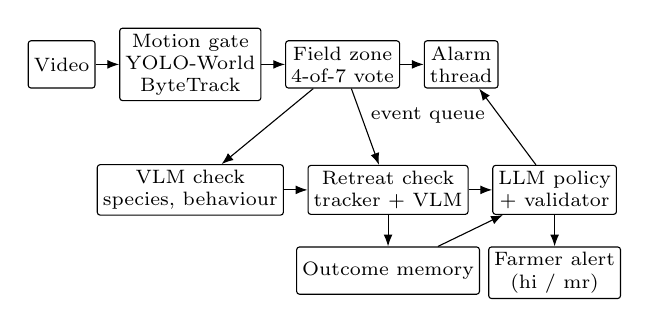
\begin{tikzpicture}[font=\scriptsize, node distance=3mm and 3mm,
  b/.style={draw, rounded corners=1pt, align=center, minimum height=6mm, inner sep=2pt},
  a/.style={-{Latex[length=1.5mm]}}]
\node[b] (v) {Video};
\node[b, right=of v] (d) {Motion gate\\YOLO-World\\ByteTrack};
\node[b, right=of d] (z) {Field zone\\4-of-7 vote};
\node[b, right=of z] (al) {Alarm\\thread};
\draw[a] (v) -- (d); \draw[a] (d) -- (z); \draw[a] (z) -- (al);
\node[b, below=8mm of d] (vl) {VLM check\\species, behaviour};
\node[b, right=of vl] (r) {Retreat check\\tracker + VLM};
\node[b, right=of r] (p) {LLM policy\\+ validator};
\node[b, below=4mm of r] (m) {Outcome memory};
\node[b, below=4mm of p] (n) {Farmer alert\\(hi / mr)};
\draw[a] (z) -- node[right, pos=0.35]{event queue} (r);
\draw[a] (z) -- (vl);
\draw[a] (vl) -- (r); \draw[a] (r) -- (p); \draw[a] (p) -- (al);
\draw[a] (r) -- (m); \draw[a] (p) -- (n); \draw[a] (m) -- (p);
\end{tikzpicture}
\caption{Two-speed architecture. The top row runs on every frame with no network and no LLM; the agent
below handles each event without ever blocking it.}\label{fig:arch}
\end{figure}

\todo{Fast path; agent; prompt rules R1--R6 (farmguard/agent/prompts.py); validator; non-GenAI fallback
for every step. Add the event sequence figure (plan Figure 2). State humane deterrents only.}

\section{Experimental Setup}
\subsection{Data and labelling}
\todo{Sources and licences. Split by clip, dev/test. Two labellers: report Cohen's kappa. Report day and
night separately; report any synthetic data separately from real data.}

\subsection{Models}
\todo{Detector weights, VLM and LLM ids and versions (Qwen2.5-VL~\cite{bai2025qwen}, YOLO-World~\cite{cheng2024yoloworld},
ByteTrack~\cite{zhang2021bytetrack}), hardware.}

\subsection{Simulator}\label{sec:sim}
Recorded video cannot react to a sound, so E4 simulates the response while running the same policy,
validator and memory code as the live system. The flee probability of a sound $s$ for species $k$ is
\begin{equation}
p = p_0(k,s)\, e^{-h\left(E_{k,s} + c \sum_{s'\neq s} E_{k,s'}\right)}\, m_{\mathrm{eat}}\, m_{\mathrm{night}}\, m_{\mathrm{group}},
\end{equation}
where exposures $E$ decay with a 72\,h time constant. \textbf{Every parameter is an assumption, not a
measurement}, and no result here is field data. All policies see the same events and the same outcome
noise: one pre-drawn threshold per event and attempt.

The model has known limits, and these shape the results. Retreat verification and behaviour are perfect in
simulation. No modifier depends on which sound is played, so behaviour context cannot help any policy
choose, and this simulator cannot show a benefit from VLM behaviour. Every event ends in success or escalation,
so escalation rate is one minus success rate, and time in field is dominated by the assumed
900\,s farmer arrival. With $c=0$, habituation to one sound does not carry to others, which rewards any rotating
policy over the fixed one by construction; the sensitivity grid therefore varies $c$ as well as $h$,
the effectiveness model and the eating penalty.

Events within a run share habituation state and are not independent, so the primary test is a
sign-flip test on per-run differences, Holm-adjusted. Pooled McNemar and Wilson intervals are
reported as descriptive only.

\section{Results}
\subsection{E1: Does the agent delay the alarm?}
\inputtable{e1}
\inputfigure{e1_latency}{Frame read to alarm start, agent off and on.}{}
\todo{Interpret from the median difference and its CI, plus per-frame detector time under VLM load; a
non-significant test alone does not show ``unchanged''.}

\subsection{E2: Can a VLM read species and behaviour?}
\IfFileExists{tables/e2_ollama-qwen2.5vl-7b.tex}{\input{tables/e2_ollama-qwen2.5vl-7b.tex}}{\todo{E2 table: needs labels and a VLM}}
\todo{Interpret; report raw accuracy and accuracy when committed.}

\subsection{E3: Can we tell if it left?}
\IfFileExists{tables/e3_ollama-qwen2.5vl-7b.tex}{\input{tables/e3_ollama-qwen2.5vl-7b.tex}}{\todo{E3 table: needs labels and a VLM}}

\subsection{E4: Does adaptation help? (simulated)}
\inputtable{e4_random}
\inputtable{e4_random_tests}
\inputtable{e4_informed}
\inputtable{e4_informed_tests}
\inputfigure{e4_learning_curves}{Simulated success rate over time, mean and standard error across runs. Assumptions, not field data.}{*}
\inputfigure{e4_time_in_field}{Simulated mean time in field. Dominated by the assumed farmer arrival time.}{*}
\inputfigure{e4_sensitivity}{Simulated success rate, marginal over the other factors of the sensitivity grid.}{*}
\inputtable{e4_grid}

Among the non-GenAI baselines, learning from outcomes added little over random rotation. The two are tied
in the base scenario, and across the 36-cell grid the bandit's mean advantage is under one percentage
point: significant in 13 cells, never above 4 points. The gain over the fixed policy comes mostly
from rotation itself, and it shrinks sharply when habituation carries across sounds ($c=0.5$), the
case the base scenario assumes away. \todo{Add the LLM column and compare; report it
even if it loses to the bandit or to random. Check the wording against the final tables.}

\subsection{E5: Fewer false alarms?}
\IfFileExists{tables/e5_ollama-qwen2.5vl-7b.tex}{\input{tables/e5_ollama-qwen2.5vl-7b.tex}}{\todo{E5 table: needs clips, intervals and a VLM}}

\subsection{E6: Better farmer alerts?}
\inputtable{e6}
\todo{Blind rating by 10+ raters, farmers if possible. Example alerts (plan Figure 8) need Devanagari support: switch to XeLaTeX or include as images.}

\subsection{Cost of the agent}
\todo{VLM latency per event, local vs cloud; LLM calls per event; invalid-action rate before the validator.}

\section{Discussion}
\todo{Limits: simulated deterrence, small data, synthetic placeholder sounds that are not claimed to deter.
Deployment path: ESP32 speakers, solar. Field trial as future work.}

Ethics: humane deterrents only, with no harm devices; people in frames are never sent to cloud APIs; farmer
data stays local; synthetic sounds are placeholders and are not claimed to deter.

\section{Conclusion}
\todo{Write after results.}

\bibliographystyle{IEEEtran}
\bibliography{refs}

\end{document}
